\TransitionFrame{utilizzi in campo medico}

\begin{frame}{Alcune applicazioni in campo medico}
\begin{columns}
\begin{column}{0.5\textwidth}
\begin{itemize}
    \item<1-> neurochirurgia
    \begin{itemize}
        \item<2-> somministrazione intracerebrale di farmaci
        \item<3-> rimozione di emorragie
    \end{itemize}
    \item<4-> otorinolaringoiatria
    \begin{itemize}
        \item<5-> Functional Endoscopic Sinus Surgery
        %\item<6-> chirurgia della gola
    \end{itemize}
    \item<6-> cardiochirurgia
    \begin{itemize}
        \item<6-> chirurgia intracardiaca per via percutanea
    \end{itemize}
    %\item<7-> chirurgia vascolare
    \item<7-> ...
\end{itemize}
\end{column}
\begin{column}{0.8\textwidth}
\only<1>{\hspace*{1em}
\includegraphics[height=0.7\textheight]{slide_uso/uso_neuro.png}}
\only<2>{\hspace*{1em}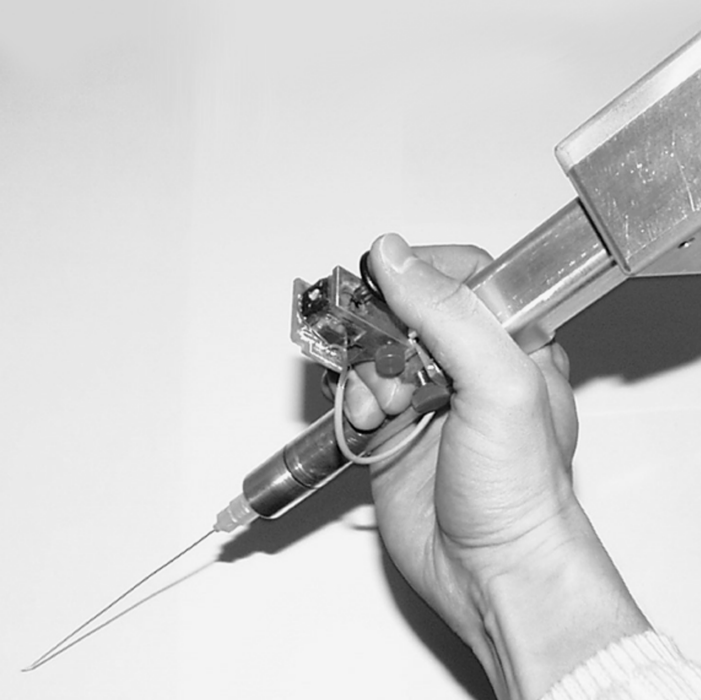
\includegraphics[height=0.7\textheight]{slide_uso/uso_neuro_drugdelivery.png}}
\only<3>{\hspace*{1em}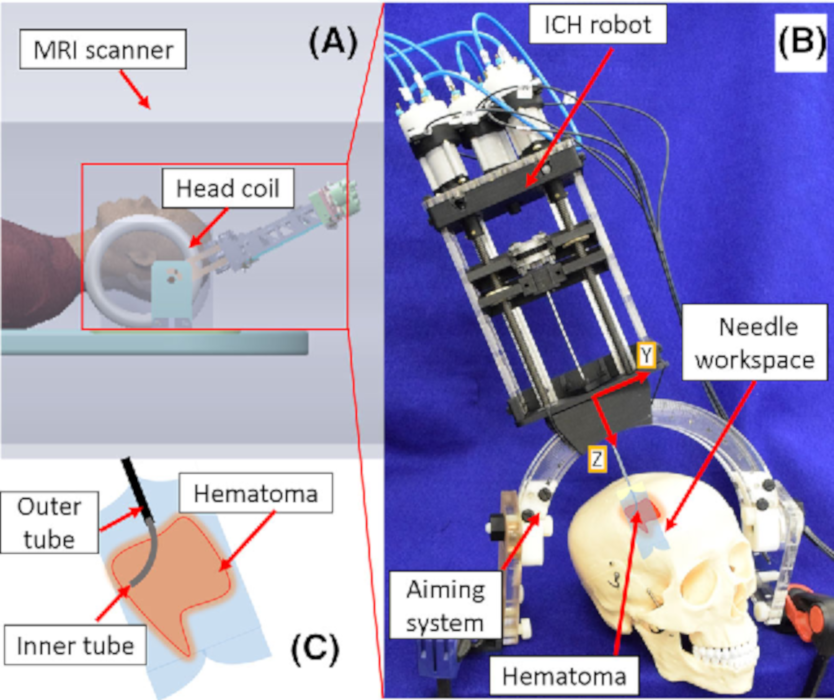
\includegraphics[height=0.7\textheight]{slide_uso/uso_neuro_hematoma.png}}
\only<4>{\hspace*{1em}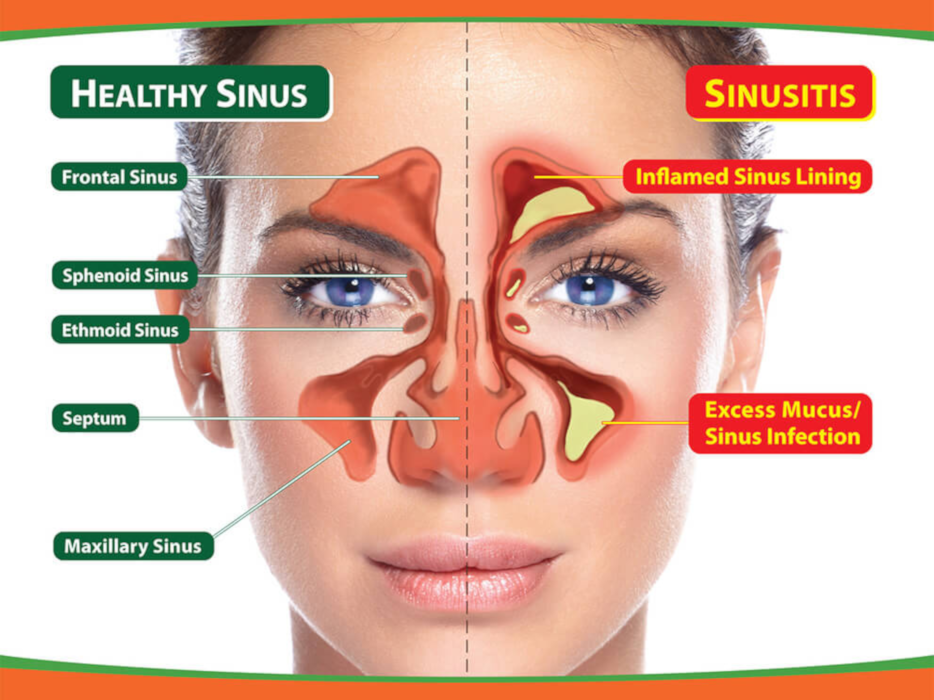
\includegraphics[height=0.7\textheight]{slide_uso/usi_otorinolaringoiatria.png}}
\only<5>{\hspace*{1em}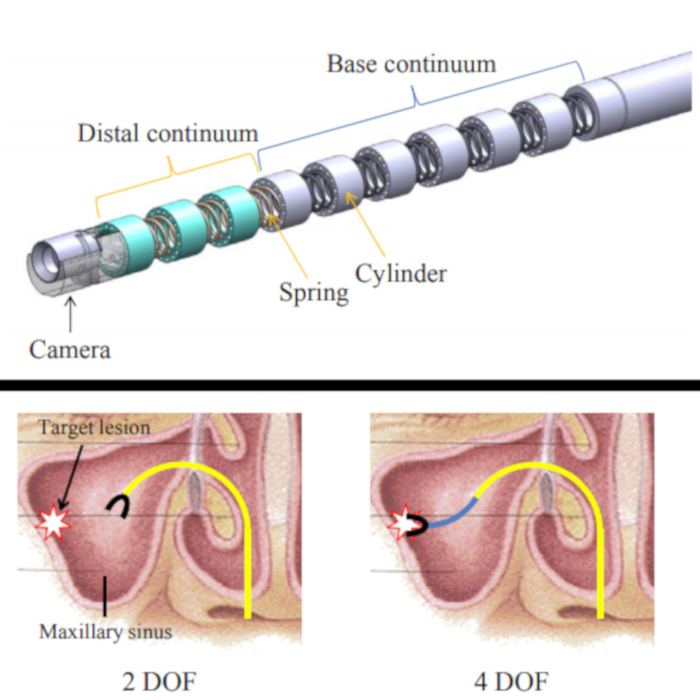
\includegraphics[height=0.7\textheight]{slide_uso/uso_otorino_fess.png}}
%\only<6>{\hspace*{1em}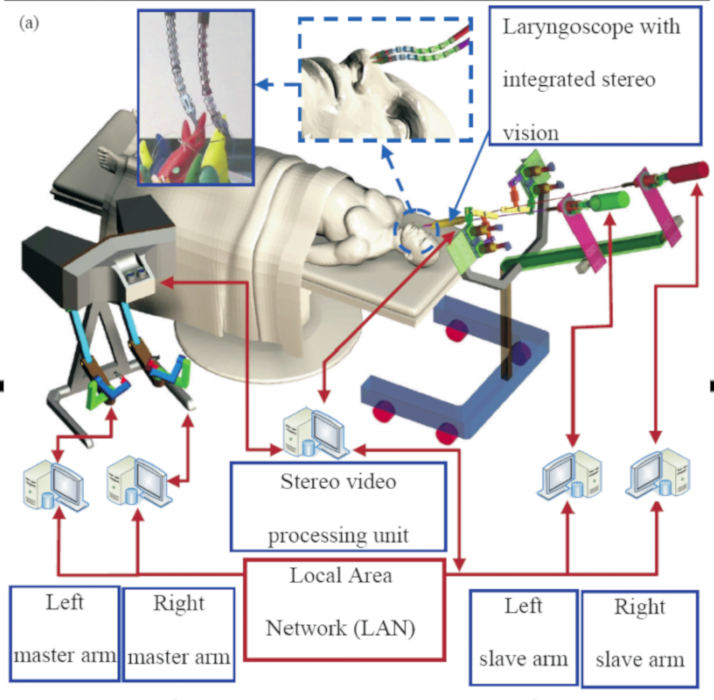
\includegraphics[height=0.7\textheight]{slide_uso/uso_otorino_throat.png}}
\only<6>{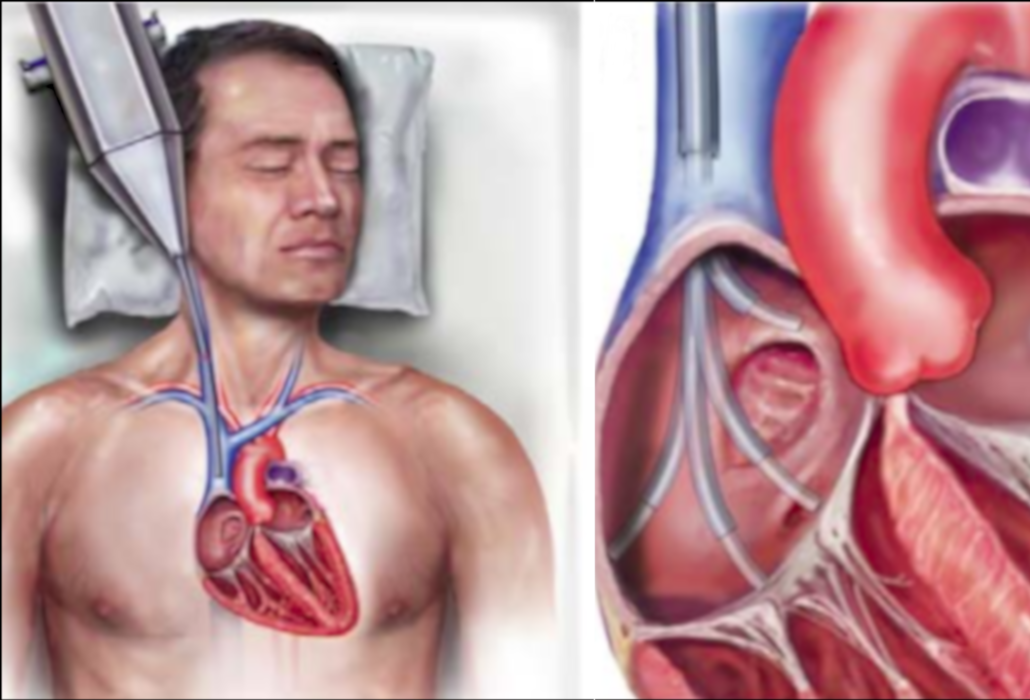
\includegraphics[height=0.7\textheight]{slide_uso/uso_cardio.png}}
\only<7>{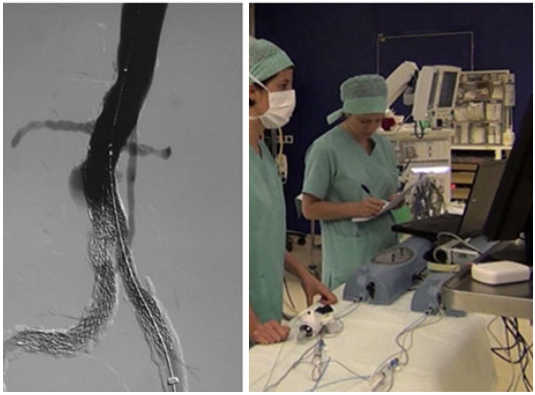
\includegraphics[height=0.7\textheight]{slide_uso/uso_vascolare.png}}
\end{column}
\end{columns}
\only<2>{\Reference{Design choices in needle steering: A review}{Van der Berg et al.}{2015}}
\only<3>{\Reference{Debulking From Within: A Robotic Steerable Cannula for Intracerebral Hemorrhage Evacuation}{Burgner et al.}{2013}}
\only<5>{\Reference{Compact Design of a Dual Master-Slave System for Maxillary Sinus Surgery}{Yoon et al.}{2013}}
%\only<6>{\Reference{Design and Integration of a Telerobotic System for Minimally Invasive Surgery of the Throat}{Simaan, Xu, Wei}{2009}}
\only<6>{\Reference{Percutaneous Steerable Robotic Tool Delivery Platform and Metal Microelectromechanical Systems Device for Tissue Manipulation and Approximation}{Vasiyev et al.}{2013}}
%\only<7>{\Reference{Current and Emerging Robot-Assisted Endovascular Catheterization Technologies: A Review}{Rafii-Tari, Payne, Yang}{2013}}

\note{
Neurochirurgia rischi $\to$ grandi aperture, spostamento dei tessuti per raggiungere regioni più profonde. 

Neurochirurgia: somministrazione intracerebrale farmaci $\to$ manipolatori tip steereble needle (punta orientabile) portano l'ago nell'esatta posizione, possono essere costrutiti tramite tubi concentrici. 

Neurochirurgia: rimozione emorragie $\to$ manipolatore a (due) tubi concentrici. Quello esterno diritto raggiunge il luogo. Quello interno, curvo, è interscambiabile per raggiunge coaguli di forme e dimensioni diverse.

Otorino-laringo-iatria $\to$ (zona orecchie naso gola) Parte superiore ed inferiore seno mascellare difficili da raggiungere.  Endoscopio 4 gdl (2+2 prossimale+distale) supera le limitazioni di quello classico diritto. 

Cardiochirurgia rischi $\to$ operazioni a cuore aperto, operazioni senza battito. 
Proposta di operazione al cuore $\to$ attraverso catetere = manipolatore composto da parte prossimale per raggiungere il luogo e distale per manipolare i tessuti, implementato tramite tubi concentrici per il loro diametro ridotto.
}
\end{frame}